%%%%%%%%%%%%%%%%%%%%%%%%%
%% C O M P A R A T O R %%
%%%%%%%%%%%%%%%%%%%%%%%%%

\subsection{Comparator}
\label{subsec:comparator}

The Comparator module is responsible for determining whether the requested tag is present in the selected cache set. The module receives the requested tag and the array of tags corresponding to all ways of the selected set from the Tag Memory.

\begin{figure}[h]
	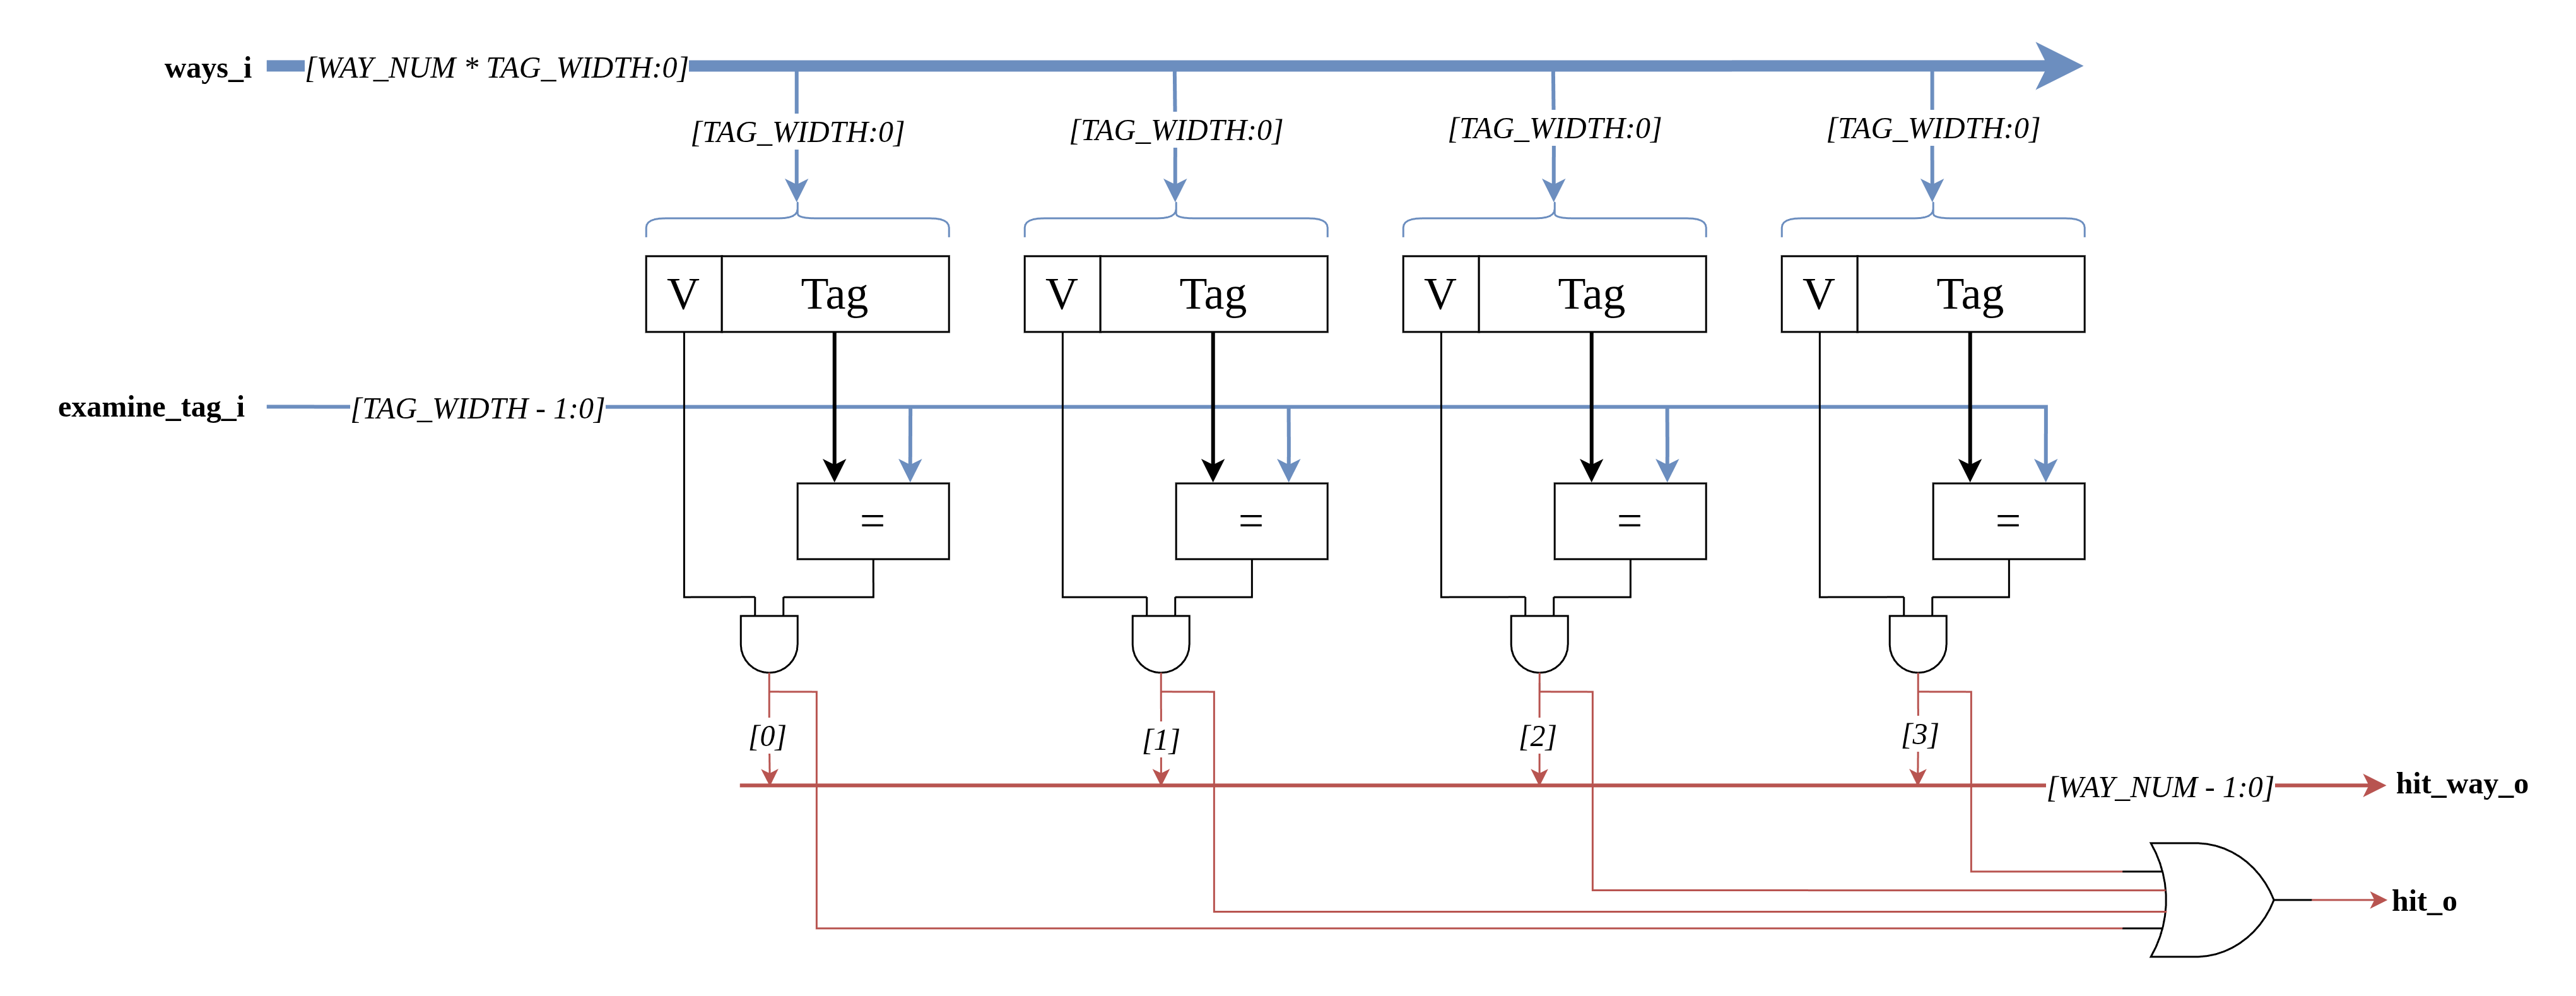
\includegraphics[width=16cm]{Comparator.png}
	\caption{Comparator scheme (4-way cache)}
\end{figure}

The comparison is performed in parallel. For each way, a dedicated comparator compares the tag stored in the corresponding way with the requested tag. The results of the individual comparisons form a match vector. Each bit of this vector corresponds to one way and is asserted when the tag stored in the corresponding way matches the requested tag. Thus, the output of the module represents the location of the matching tag using a one-hot encoding.

\begin{table}[htbp]
	\centering
	\small
	\begin{tabularx}{\textwidth}{l c c X}
		\toprule
		\textbf{Parameter} & \textbf{Valid Range} & \textbf{Default} & \textbf{Description} \\
		\midrule
		
		\verb|TAG_WIDTH| &
		Positive integer &
		--- &
		Width of the cache tag. \\
		
		\verb|WAY_NUM| &
		Positive integer &
		--- &
		Number of cache ways compared in parallel. \\
		
		\bottomrule
	\end{tabularx}
	\caption{Comparator parameters}
	\label{tab:comparator_parameters}
\end{table}

\begin{table}[htbp]
	\centering
	\label{tab:comparator_ports}
	\small
	\begin{tabularx}{\textwidth}{l c c X}
		\toprule
		\textbf{Ports} & \textbf{Direction} & \textbf{Width} & \textbf{Description} \\
		\midrule
		\verb| ways_i | & Input & \verb| WAY_NUM * (TAG_WIDTH + 1) | & Tags and valid bits of all ways belonging to the selected set. \\
		\verb| examine_tag_i| & Input & \verb| TAG_WIDTH | & Tag of the requested cache line to be compared against all ways. \\
		\verb| hit_way_o | & Output & \verb| WAY_NUM | & One-hot encoded indication of the way containing the requested tag.. \\
		\verb| hit_o | & Output & \verb| 1 | & Indicates whether the requested tag was found in any way of the selected set. \\
		\bottomrule
	\end{tabularx}
	\caption{Comparator ports}
\end{table}